\selectlanguage{ngerman}%
\frenchspacing%
\begin{ledgroupsized}[r]{120mm}%
\footnotesize%
\pstart%
\noindent\textbf{Überlieferung:}
\pend%
\end{ledgroupsized}%
\begin{ledgroupsized}[r]{114mm}%
\footnotesize%
\pstart%
\parindent -6mm%
\makebox[6mm][l]{\textit{L}}%
Aufzeichnung:
LH XXXV 10,\;13 Bl.\;8.
Ein Zettel (etwa 10\;x\;21~cm),
Ränder zum Teil beschnitten oder abgerissen.
Eineinhalb Seiten (sonst unbeschrieben).
\pend%
\end{ledgroupsized}%
\selectlanguage{latin}%
\frenchspacing%
\vspace{8mm}%
\normalsize%
\pstart%
\noindent%
\lbrack%
\href{\Scan{LH_35_10_13_008r}}%
{8\,r\textsuperscript{o}}%
\rbrack%
\hfill%
Concursus Eccentrici%
\indexS{concursus eccentricus}
casus simplicissimus%
\indexS{casus simplex}
\hfill%
\phantom{\lbrack8\:r\textsuperscript{o}\rbrack}%
\par%
\centering%
Scheda 2%
\indexS{scheda}
\quad%
\edlabel{LH_35_10_13_008_008r_datum-1}%
Septemb.\;691%
\edlabel{LH_35_10_13_008_008r_datum-2}
\pend%
\vspace{1.0em}
\pstart%
\noindent%
Si aequales
\edtext{et parallelae rectae%
\indexS{rectae parallelae}%
}{%
\lemma{et}\Bfootnote{%
parallelae rectae
\textit{erg.\;L}}}
\textit{AB}, \textit{LM}
concurrant in plano paginae%
\indexS{planum paginae}%
\indexS{pagina}
partibus \textit{BC}, \textit{MN},
celeritate aequali,%
\indexS{celeritas concursus}
is est casus simplicissimus%
\indexS{casus simplex}
Concursus Eccentrici,%
\indexS{concursus eccentricus}
et fit utrobique idem.
Videndum an liceat rem ita concipere,
quasi concurrerent solum partes
\textit{BC} %
et \textit{MN} %
atque ita reflecterentur%
\lbrack,\rbrack\
in momento autem reflexionis%
\indexS{reflexio}%
\indexS{momentum reflexionis}
invenirent illa \textit{AC}, haec \textit{LN}
venientes contra reflexionem%
\indexS{reflexio}
et ipsis \textit{BC}, \textit{MN}
\edtext{adhaerescentes.
Quo admisso}{%
\lemma{adhaerescentes.}\Bfootnote{%
\textit{(1)}~Quod
\textit{(2)}~Quo admisso%
~\textit{L}}}
jam in sola \textit{AB} considerare licet %
quid fiat
si duo cohaerescant,
\textit{AC} tendens prorsum
et \textit{BC} retrorsum.
Quo
\edtext{posito fiet gyratio.%
\indexS{gyratio in concursu eccentrico}
Sumamus partem%
}{%
\lemma{posito}\Bfootnote{%
\textit{(1)}~pars i
\textit{(2)}~fiet gyratio. Sumamus partem%
~\textit{L}}}
\textit{AF} aequalem ipsi \textit{BC},
hae duae conspirabunt in gyrationem%
\indexS{conspiratio in gyratione}
circa medium \textit{E}.
Perinde ergo est
ac si simul cohaerescerent
\edtext{\lbrack\textit{AF}\rbrack}{%
\lemma{\textit{AC}}\Bfootnote{%
\textit{L~ändert Hrsg.}}}
tendens prorsum,
\textit{BC} retrorsum,
\textit{CF} prorsum.
Ubi
\edtext{\lbrack nisus\rbrack}{%
\lemma{nisus}\Bfootnote{%
\textit{gestr.\;L, wieder gültig macht Hrsg.}}}
ipsorum \textit{AF} et \textit{BC}
conspirat in circulationem,%
\indexS{circulatio in concursu eccentrico}%
\indexS{conspiratio in circulatione}
nisus ipsius \textit{CF} residui%
\indexS{nisus residui}
proficit in totius progressionem.%
\indexS{progressio totius}
\pend%
\vspace{2.75em}%
\centerline{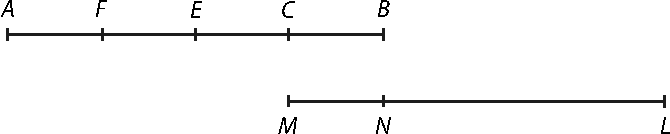
\includegraphics[width=0.74\textwidth]{gesamttex/edit_VIII-4/images/LH_35_10_13_008_d1_008r.pdf}}
\vspace{1.5em}
\centerline{\lbrack\textit{Fig.\:1}\rbrack}
\newpage%
\pstart%
\edlabel{LH_35_10_13_008_008r_gedankenexp-1}%
Possumus autem examinare Nisum%
\indexS{nisus}
per conatum.%
\indexS{conatus}
\edtext{Fingamus Cylindrum%
\indexS{cylinder in aqua}
in aqua poni \textit{AB},
compositum ex duabus partibus%
}{%
\lemma{Fingamus}\Bfootnote{%
\textit{(1)}~duas esse pa
\textit{(2)}~Cylindrum in %
\lbrack...\rbrack\ duabus partibus%
~\textit{L}}}
\textit{AC} et \textit{BC},
quarum una sit gravis altera levis,
ita ut levitas%
\indexS{levitas specifica}
\edtext{speci\lbrack fi\rbrack ca}{%
\lemma{specica}\Bfootnote{%
\textit{L~ändert Hrsg.}}}
sit aequalis gravitati specificae,%
\indexS{gravitas specifica}
seu in casu aequalium molium%
\indexS{moles aequales}
et situs directi%
\indexS{situs}
altera alteri
\edtext{resistat.
Videndum tuncne}{%
\lemma{resistat.}\Bfootnote{%
\textit{(1)}~Ita fingendum est
\textit{(2)}~Videndum tuncne%
~\textit{L}}}
centrum gravitatis aquae%
\indexS{centrum gravitatis aquae}
considerandum,
ut quam maxime descendat totius centrum%
\indexS{centrum gravitatis totius}
ex aqua et corpore compositi,
an abstrahendo animum%
\indexS{animus}
ab aqua%
\indexS{aqua}
liceat definire modum
quo quam brevissime natura lucratur%
\indexS{natura lucrans}
quantum potest,
ut scilicet et progressionem%
\indexS{progressio in concursu eccentrico}
et circulationem%
\indexS{circulatio in concursu eccentrico}
hac arte%
\indexS{ars}
definiamus.
Apparebit enim
quomodo conatus inter ipsas sit
\edtext{dividendus.%
\indexS{conatus dividendus}
Quam optime procedamus.}{%
\lemma{dividendus.}\Bfootnote{%
\textit{(1)}~, vel
\textit{(2)}~. Quam optime procedamus.%
~\textit{L}}}%
\edlabel{LH_35_10_13_008_008r_gedankenexp-2}%
\pend%
\pstart%
\edlabel{LH_35_10_13_008r_kehg-1}%
Quid si ab initio concepissemus %
obniti sibi
\edtext{duo aequalis gravitatis%
\indexS{gravitas specifica}
et levitatis specificae,%
\indexS{levitas specifica}
\!\textit{AB} grave
et
\lbrack\textit{LM}\rbrack\
leve;
sed}{%
\lemma{duo}\Bfootnote{%
\textit{(1)}~sed
\textit{(2)}~aequalis gravitatis %
\lbrack...\rbrack\ grave et
\bars{\textit{BC} \textit{ändert Hrsg.}}
leve; sed%
~\textit{L}}}
tunc periret vis%
\indexS{vis ictus}
\edtext{ictus,%
\indexS{ictus}
quia \textit{BC} et
\lbrack\textit{MN}\rbrack\
se non repellerent%
\lbrack;\rbrack\
verum ita circulatio%
\indexS{circulatio in concursu eccentrico}
fieret aliter et satis curiose,%
}{%
\lemma{ictus,}\Bfootnote{%
\textit{(1)}~et ita aliter se haberet circulatio
\textit{(2)}~quia \textit{BC} et
\bars{\textit{LN} \textit{ändert Hrsg.}}
se non %
\lbrack...\rbrack\ satis curiose,%
~\textit{L}}}
conabitur enim \textit{AB} gyrare circa punctum
\edtext{\lbrack\textit{M}\rbrack,}{%
\lemma{\textit{L}}\Bfootnote{%
\textit{L~ändert Hrsg.}}}
et \textit{LM}
\edlabel{35_10_13_008r_1a}%
super punctum \textit{B}.%
\edtext{}{%
\xxref%
{35_10_13_008r_1a}{35_10_13_008r_1b}%
\lemma{super}\Bfootnote{%
punctum
\bars{super \textit{streicht Hrsg.}}
\textit{B}. \lbrack/\rbrack\
\textit{(1)}~Vis respectiva
\textit{(2)}~Vis quam habet motus
\textit{(a)}~circulat\textlangle ar\textrangle\
\textit{(b)}~\bars{circulatoribus \textit{ändert Hrsg.}} et vis %
\lbrack...\rbrack\ motus progressorius%
~\textit{L}}}%
\pend%
\pstart%
Vis%
\indexS{vis motus circulatorii}
quam habet motus%
\indexS{motus circulatorius}
circulatori\lbrack us\rbrack\
et vis%
\indexS{vis motus progressorii}
quam habet motus progressorius%
\indexS{motus progressorius}%
\edlabel{35_10_13_008r_1b}
ipsius \textit{AB},
inter se sunt conjungendae;%
\indexS{vires conjungendae}
debet enim oriri aequatio\indexS{aequatio}
seu compensatio,\indexS{compensatio}
seu idem
\edtext{quod}{%
\lemma{\textit{Am Rand:}}\Afootnote{NB}}
prodiret
\edtext{aestimati\lbrack s\rbrack}{%
\lemma{aestimatibus}\Bfootnote{%
\textit{L~ändert Hrsg.}}}
viribus%
\indexS{vis aestimata}
cujusque puncti ex motu composito,%
\indexS{motus compositus}%
\indexS{aestimatio virium ex motu composito}
prorsus ut in compositione cum
\edlabel{LH_35_10_13_008r_iugl-1}%
navi.%
\indexS{compositio cum navi}\indexS{navis}%
\edlabel{LH_35_10_13_008r_kehg-2}%
\edtext{}{%
\xxref{LH_35_10_13_008r_iugl-1}{LH_35_10_13_008r_iugl-2}%
\lemma{navi.}\Bfootnote{%
\lbrack/\rbrack\
\textit{(1)}~Si \textit{L}
\textit{(a)}~glo
\textit{(b)}~globus\indexS{globus}
\textit{(2)}~Si \textit{L} globulus%
~\textit{L}}}%
\pend%
\vspace{2.75em}%
\centerline{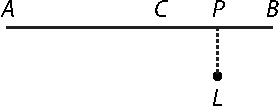
\includegraphics[width=0.33\textwidth]{gesamttex/edit_VIII-4/images/LH_35_10_13_008_d2_008v.pdf}}
\vspace{1.0em}
\centerline{\lbrack\textit{Fig.\:2}\rbrack}
\vspace{1.5em}%
\pstart%
Si \textit{L} globulus%
\indexS{globulus}%
\edlabel{LH_35_10_13_008r_iugl-2}
in cylindrum \textit{AB}%
\indexS{cylinder}
directe sed eccentrice occurrat,%
\indexS{concursus directus eccentricus}%
\indexS{concursus eccentricus directus}
tunc
(\protect\vphantom)%
si verum est
quod ictus\indexS{ictus}
solum fiat
inter \textit{L} et ipsi aequalem \textit{BC}%
\protect\vphantom()
tunc si motus est aequalis %
\indexS{motus aequalis}
et%
\lbrack,\rbrack\
posito puncto incursus \textit{P},%
\indexS{punctum incursus}%
\indexS{incursus}
dupla ipsius \textit{BP},
seu \textit{BC},
aequalis est ipsi \textit{L},
debet \textit{L} semper reflecti;
hoc dignum experimento.%
\indexS{experimentum}
Cum ita \textit{L} et \textit{AB} sint inaequales%
\lbrack,\rbrack\
\edlabel{LH_35_10_13_008_008rv_navisficta-1}%
videamus quid fiat
si navem fingamus%
\indexS{navis ficta}%
\indexS{fictio navis}
et motum
\lbrack%
\href{\Scan{LH_35_10_13_008v}}%
{8\,v\textsuperscript{o}}%
\rbrack\ %
inter ipsa reciprocum molibus,%
\indexS{motus reciprocus moli}%
\indexS{moles reciproca motui}
et quae deinde prodeant
inter \textit{L} et \textit{BC},
quorum ita celeritas non erit
reciproca molibus nec aequalibus.%
\indexS{celeritas reciproca moli}%
\indexS{moles reciproca celeritati}
Utile erit varias hypotheses%
\indexS{hypotheses comparatae}%
\indexS{comparatio hypothesum}
comparare inter se,
debent enim omnes dare idem,
navis utcunque assumto motu%
\indexS{navis}%
\indexS{motus navis}%
\lbrack;\rbrack\
in quo latent quaedam subtilia.%
\edlabel{LH_35_10_13_008_008rv_navisficta-2}
\pend%
\pstart%
Datur et modus omnia definiendi,%
\indexS{modus definiendi}
si fingamus
corpora constare meris globis aequalibus%
\indexS{corpus constans globis aequalibus}
connexis per elastra,%
\indexS{globi connexi per elastra}%
\indexS{connexio per elastra}%
\indexS{elastrum}
quae sine tensione%
\indexS{tensio}
nec distrahi invicem,%
\indexS{distractio cum tensione}
nec contrudi patiantur.%
\indexS{contrusio cum tensione}
Ita plurima definire poterunt Geometrice.%
\indexS{definitio geometrica}
Et consensus haberi debet%
\indexS{consensus}
cum iis quae jam habemus.
Ita ex solis legibus globulorum aequalium%
\indexS{lex globorum aequalium}%
\indexS{globi aequales}
caetera definientur.
\pend%
\selectlanguage{latin}%
\frenchspacing%
\normalsize%
